\documentclass[draft, twocolumn]{article}
\usepackage[unicode,draft=false,hidelinks]{hyperref}
\usepackage{cite}
\usepackage{catchfilebetweentags}
\usepackage{amssymb}
\usepackage{turnstile}
\usepackage{bbm}
\usepackage[greek, english]{babel}
\usepackage{MnSymbol}
\usepackage{stmaryrd}
\usepackage{csquotes}
\newcommand\doubleplus{+\kern-1.3ex+\kern0.8ex}
\newcommand\mdoubleplus{\ensuremath{\mathbin{+\mkern-8mu+}}}
\makeatletter
\newcommand\incircbin
{%
  \mathpalette\@incircbin
}
\newcommand\@incircbin[2]
{%
  \mathbin%
  {%
    \ooalign{\hidewidth$#1#2$\hidewidth\crcr$#1\bigcirc$}%
  }%
}
\newcommand{\oeq}{\ensuremath{\incircbin{=}}}
\makeatother
\usepackage{ucs}
\DeclareUnicodeCharacter{8759}{\ensuremath{\squaredots}}
\DeclareUnicodeCharacter{951}{\textgreek{\texteta}}
\DeclareUnicodeCharacter{737}{\ensuremath{^\text{l}}}
\DeclareUnicodeCharacter{691}{\ensuremath{^\text{r}}}
\DeclareUnicodeCharacter{7523}{\ensuremath{_\text{r}}}
\DeclareUnicodeCharacter{8718}{\ensuremath{\blacksquare}}
\DeclareUnicodeCharacter{957}{\textgreek{\textnu}}
\DeclareUnicodeCharacter{961}{\textgreek{\textrho}}
\DeclareUnicodeCharacter{929}{\textgreek{\textRho}}
\DeclareUnicodeCharacter{954}{\textgreek{\textkappa}}
\DeclareUnicodeCharacter{10214}{\ensuremath{\lsem}}
\DeclareUnicodeCharacter{10215}{\ensuremath{\rsem}}
\DeclareUnicodeCharacter{8857}{\mdoubleplus}
\DeclareUnicodeCharacter{8860}{\oeq}
\DeclareUnicodeCharacter{9043}{\ensuremath{\triangle}}
\DeclareUnicodeCharacter{928}{\textgreek{\textPi}}
\DeclareUnicodeCharacter{922}{\textgreek{\textKappa}}
\DeclareUnicodeCharacter{931}{\textgreek{\textSigma}}
\DeclareUnicodeCharacter{916}{\textgreek{\textDelta}}
\DeclareUnicodeCharacter{8779}{\ensuremath{\backtriplesim}}
\DeclareUnicodeCharacter{8799}{\ensuremath{\stackrel{?}{=}}}
\DeclareUnicodeCharacter{10181}{\ensuremath{\lbag}}
\DeclareUnicodeCharacter{10182}{\ensuremath{\rbag}}
\usepackage[utf8x]{inputenc}
\usepackage[T1]{fontenc}
\usepackage{autofe}
\usepackage[references]{agda}
\usepackage{bbding}
\setlength{\marginparwidth}{2cm}
\usepackage[obeyDraft]{todonotes}
\usepackage{lineno}
\setlength\linenumbersep{-0.5cm}
\usepackage{amsthm}
\theoremstyle{definition}
\newtheorem{definition}{Definition}[section]
\theoremstyle{remark}
\newtheorem{principle}{Principle}[section]
\usepackage{subcaption}
\usepackage{graphicx}
\usepackage{tikz}
\usetikzlibrary{decorations.pathmorphing}
\usetikzlibrary{snakes}
\usetikzlibrary{arrows}
\usetikzlibrary{cd}
\usepackage{forest}
\author{Donnacha Oisín Kidney}
\title{Automatically And Efficiently Illustrating Polynomial Equalities in Agda}
\begin{document}
\maketitle
\begin{abstract}
  We present a new library which automates the construction of equivalence
  proofs between polynomials over commutative rings in the programming language
  Agda\cite{norell_dependently_2008}. The library makes use of Agda's reflection
  machinery to provide an extremely simple interface, and is extremely flexible
  in its output, requiring only equivalence (not propositional equality) to
  construct proofs.
\end{abstract}


  % The underlying algorithm is the same as
  % that in Coq's\cite{the_coq_development_team_2018_1219885} \verb+ring+ tactic
  % \cite{gregoire_proving_2005}.


  

  % We demonstrate techniques for constructing proofs based on the theory of
  % lists, show how Agda's reflection system can be used to provide a safe and
  % simple interface to the solver, and compare the ``correct by construction''
  % approach to that of auxiliary proofs.
  
  % We also show that, as a by-product of proving equivalences rather than
  % equalities, the prover can be used to provide artifacts other than equational
  % proofs, including step-by-step solutions, and isomorphisms.
\tableofcontents
\section{Introduction}
Truly formal proofs of even basic mathematical identities are notoriously
tedious and verbose. Perhaps the canonical example is Russell and Whitehead's
proof that \(1+1=2\), which finally arrives on page 379 of Principia
Mathematica\cite{whitehead_principia_1910}. 

More modern systems have greatly simplified the underlying formalisms, but they
still often suffer from a degree of explicitness that makes elementary
identities daunting. Dependently-typed programming languages like
Agda\cite{norell_dependently_2008} and
Coq\cite{the_coq_development_team_2018_1219885} are examples of such systems:
used in the naïve way, equivalence proofs require the programmer to specify
every individual step (``here we rely on the commutativity of \(+\), followed by
the associativity of \(\times\) on its right side'', and so on).

Coq and Agda are not just programming languages in name, though: they are
fully-fledged and powerful, capable of producing useful software, including
automated computer-algebra systems. Unlike most CASs, those written in Coq or
Agda come with added guarantees of correctness in their operation. Furthermore,
these systems can be used to automate the construction of identity proofs which
would otherwise be too tedious to do by hand.
\section{Related Work}
The state-of-the-art solver for polynomial equalities (over commutative rings)
was originally presented in\cite{gregoire_proving_2005}, and is used in Coq's
\verb+ring+ solver. This work improved on the already existing
solver\cite{Coq:manual} in both efficiency and flexibility. In both the old and
improved solvers, a reflexive technique is used to automate the construction of
the proof obligation (as described in\cite{boutin_using_1997}).

Agda\cite{norell_dependently_2008} is a dependently-typed programming language
based on Martin-Löf's Intuitionistic Type
Theory\cite{martin-lof_intuitionistic_1980}. Its standard
library\cite{danielsson_agda_2018} currently contains a ring solver which is
similar in flexibility to Coq's \verb+ring+, but doesn't support the
reflection-based interface, and is less efficient due to its use of a dense
(rather than sparse) internal data structure.

In\cite{geuvers_automatically_2017}, an implementation of an automated solver
for the dependently-typed language Idris\cite{brady_idris_2013} is described. It
uses type-safe reflection to provide a simple and elegant interface, and its
internal solver algorithm uses a correct-by-construction approach. The solver is
defined over \emph{non}commutative rings, however, meaning that it is more
general (can work with more types) but less powerful (meaning it can prove fewer
identities). It does not use a sparse representation.

Reflection and metaprogramming are relatively recent additions to Agda, but form
an important part of the interfaces to automated proof procedures. Reflection in
dependent types in general is explored in\cite{christiansen_practical_2015}, and
specific to Agda in\cite{van_der_walt_reflection_2012}.

The progress of various formalization efforts is charted
in\cite{wiedijk_formalizing_2018}. DoCon\cite{meshveliani_docon-provable_2018}
is a notable Agda library in this regard: its implementation and goal is
described in\cite{meshveliani_dependent_2013}. \cite{cheng_functional_2018}
describes the manipulation of polynomials in both Haskell and Agda.

Finally, the study of \emph{didactic} computer algebra systems is explored
in\cite{lioubartsev_constructing_2016}.
\section{Contributions}
\begin{description}
  \item[An New, Efficient Ring Solver]
    We provide an implementation of a polynomial solver which uses the same
    optimizations described in\cite{gregoire_proving_2005} in the programming
    language Agda. Along the way, we demonstrate several techniques for writing
    efficient correct-by-construction code.
  \item[A Simple Reflection-Based Interface] We use Agda's reflection machinery
    to provide the following interface to the solver:
    \ExecuteMetaData[Contributions.tex]{lemma}
    It imposes minimal overhead on the user: only the \(\AgdaDatatype{Ring}\)
    implementation is required, with no need for user implementations of
    quoting. Despite this, it is generic over any type which implements ring.
  \item[A Didactic Computer-Algebra System] As a result of the flexibility of
    the solver, the equivalence relation it constructs can be instantiated into
    a number of different forms (not just equality, for instance). While This
    has been exploited in Agda before to generate isomorphisms over containers,
    we use it here to construct didactic (or ``step-by-step'') solutions.
\end{description}
\section{Explaining The Reflexive Technique With Monoids}
Before jumping into commutative rings, we will first illustrate a general
technique for automatically constructing equivalence proofs over a simpler
algebra---\emph{monoids}.

\begin{definition}[Monoids]
  A monoid is a set equipped with a binary operation, \(\bullet\), and a
  distinguished element \(\epsilon\), such that the following equations hold:
  \begin{align}
    x \bullet (y \bullet z) &= (x \bullet y) \bullet z \tag{Associativity} \\
    x \bullet \epsilon      &= x \tag{Left Identity} \\
    \epsilon \bullet x      &= x \tag{Right Identity}
  \end{align}
  Addition and multiplication (with 0 and 1 being the respective identity
  elements) are perhaps the most obvious instances of the algebra. In computer
  science, monoids have proved a useful abstraction for formalizing concurrency
  (in a sense, an associative operator is one which can be evaluated in any
  order).
\end{definition}
\subsection{A ``Trivial'' Identity}
\begin{figure}
  \ExecuteMetaData[Monoids.tex]{mon-ident}
  \caption{A Simple Identity Of Monoids}
  \label{mon-ident}
\end{figure}

As a running example for this section, we will use the identity in
figure~\ref{mon-ident}. To a human, the fact that the identity holds may well be
obvious: \(\AgdaField{∙}\) is associative, so we can scrub out all the
parentheses, and \(\AgdaField{ε}\) is the identity element, so scrub it out too.
After that, both sides are equal, so voilà! 

Unfortunately, our compiler isn't nearly that clever. As alluded to before, we
need to painstakingly specify every intermediate step, justifying every move:

\begin{samepage}
  \begin{linenumbers}
    \ExecuteMetaData[Monoids.tex]{mon-proof}
  \end{linenumbers}
\end{samepage}

The syntax is designed to mimic that of a handwritten proof: line 3 is the
expression on the left-hand side of \(\AgdaField{≈}\) in the type, and line 9
the right-hand-side. In between, the expression is repeatedly rewritten into
equivalent forms, with justification provided inside the angle brackets. For
instance, to translate the expression from the form on line 3 to that on line 5,
the associative property of \(\AgdaField{∙}\) is used on line 4.

One trick worth pointing out is on line 6: the \(\AgdaFunction{∙-cong}\) lifts
two equalities to either side of a \(\AgdaField{∙}\). In other words, given a
proof that \(x_1 \; \AgdaField{≈} \; x_2\), and \(y_1 \; \AgdaField{≈} \; y_2\),
it will provide a proof that \(x_1 \; \AgdaField{∙} \; y_1 \; \AgdaField{≈} \;
x_2 \; \AgdaField{∙} \; y_2\). This function needs to be explicitly provided by
the user, as we only require \(\AgdaField{≈}\) to be an equivalence relation
(not just propositional equality). In other words, we don't require it to be
substitutive.
\subsection{ASTs for the Language of Monoids}
The first hurdle for automatically constructing proofs comes from the fact that
the identity is opaque: it's hidden behind a lambda. We can't scrutinize or
pattern-match on its contents. Our first step, then, is to define an AST for
these expressions which we \emph{can} pattern-match on:

\begin{samepage}
  \ExecuteMetaData[Monoids.tex]{mon-ast}
\end{samepage}

We have constructors for both monoid operations, and a way to refer to
variables. These are referred to by their de Bruijn indices (the type itself is
indexed by the number of variables it contains). Here is how we would represent
the left-hand-side of the identity in figure~\ref{mon-ident}:
\begin{center}
  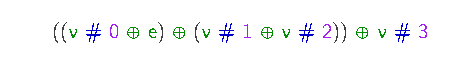
\includegraphics[draft=false]{graphics/lhs-ast}
\end{center}

To get \emph{back} to the original expression, we can write an ``evaluator'':
\ExecuteMetaData[Monoids.tex]{eval-ast}

This performs no normalization, and as such its refult is \emph{definitionally}
equal to the original expression\footnotemark:
\footnotetext{
  The type of the unnormalized expression has changed slightly: instead of being
  a curried function of \(n\) arguments, it's now a function which takes a
  vector of length \(n\). The final solver has an extra translation step for
  going between these two representations, but it's a little fiddly, and not
  directly relevant to what we're doing here, so we've glossed over it. We refer
  the interested reader to the Relation.Binary.Reflection module of Agda's
  standard library\cite{danielsson_agda_2018} for an implementation.
}
\ExecuteMetaData[Monoids.tex]{eval-nonnorm}

We've thoroughly set the table now, but we still don't have a solver. What's
missing is another evaluation function: one that normalizes.
\subsection{Canonical Forms}
In both the monoid and ring solver, we will make use of the \emph{canonical
  forms} of expressions in each algebra. Like the AST we defined above, these
canonical forms represent expressions in the algebra, however \emph{unlike} the
AST, they definitionally obey the laws of the algebra. 

For monoids, the canonical form is \emph{lists}.

\ExecuteMetaData[Monoids.tex]{list-def}

\(\AgdaField{ε}\) here is simply the empty list, and \(\AgdaField{∙}\) is
concatenation:
\ExecuteMetaData[Monoids.tex]{list-monoid}

Similarly to the previous AST, it has variables and is indexed by the number of
variables it contains. Its evaluation will be recognizable to functional
programmers:
\ExecuteMetaData[Monoids.tex]{list-eval}

And finally (as promised) the opening identity is \emph{definitionally} true
when written in this language:
\ExecuteMetaData[Monoids.tex]{list-obvious}

Now, to ``evaluate'' a monoid expression in a \emph{normalized} way, we simply
first convert to the language of lists:
\ExecuteMetaData[Monoids.tex]{ast-norm}

Or, combining both steps into one:
\ExecuteMetaData[Monoids.tex]{ast-norm-interp}
\subsection{Homomorphism}
Now we have a concrete way to link the normalized and non-normalized forms of
the expressions. A diagram of the strategy for constructing our proof is in
Figure~\ref{proof-process}. The goal is to construct a proof of equivalence
between the two expressions at the bottom: to do this, we first construct the
AST which represents the two expressions (for now, we'll assume the user
constructs this AST themselves. Later we'll see how too construct it
automatically from the provided expressions). Then, we can evaluate it into
either the normalized form, or the unnormalized form. Since the normalized forms
are syntactically equal, all we need is \(\AgdaInductiveConstructor{refl}\) to
prove their equality. The only missing part now is \(\AgdaFunction{correct}\),
which is the task of this section.

\begin{figure*}
  \makebox[\textwidth][c]{
    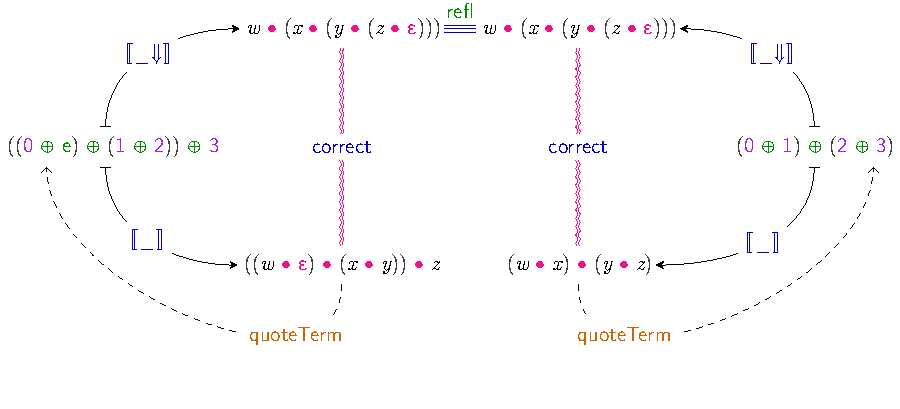
\includegraphics[draft=false]{graphics/reflexive-process}
  }
  \caption{The Reflexive Proof Process}
  \label{proof-process}
\end{figure*}
\bibliographystyle{IEEEtranS}
\bibliography{bibliography.bib}
\end{document}